\documentclass[a4paper,10pt,twocolumn]{article}

\usepackage[spanish,activeacute]{babel}
\usepackage{amsmath}
\usepackage{graphicx}

\author{Jaime P\'erez Aparicio}
\title{M\'etodos estad\'isticos en Econom\'ia y Sociolog\'ia}

\begin{document}
\maketitle

\section*{Introducci\'on}

En este proyecto he aplicado m\'etodos de la f\'isica estad\'istica a otros temas. Concretamente he usado el algoritmo de Metr\'opolis para estudiar un modelo de Potts (sistemas de varios niveles). El algoritmo de Metr\'opolis est\'a basado en el m\'etodo de Montecarlo. Voy a introducir ambos m\'etodos, pero para mejor entendimiento es preferible consultar bibliograf\'ia especializada en el tema.

\subsection*{Montecarlo}

En el m\'etodo de Montecarlo se tiene inicialmente un sistema en cierto estado. Aleatoriamente se cambia el estado de uno de los elementos que conforman al sistema. A este cambio se le asocia una puntuaci\'on. Si la puntuaci\'on es positiva o una determinada, se cambia definitivamente el sistema. Si no, se vuelve al estado anterior. 

Si se quisiera hacer una inteligencia virtual que jugara al tres en raya, el ordenador ir\'ia comprobando cada posible jugada y asign\'andole una puntuaci\'on, en funci\'on de la probabilidad que tenga esa jugada de ganar la partida. Luego escogera la que tenga m\'as puntuaci\'on. La desventaja de este m\'etodo es que tarda mucho tiempo en comprobar todos los posibles estados, lo que se puede paliar limitando el numero de estados que prev\'e. 

En este caso, el programa comprueba solo el siguiente estado, por lo que no se da el error mencionado.

\subsection*{Metr\'opolis}

La principal diferencia es que con este m\'etodo se permite al sistema ir a un estado con menor puntuaci\'on siguiendo una ley de probabilidad exponencial. Esto hace que el sistema tarde mucho m\'as en alcanzar su estado estable.

Para este trabajo se ha usado el algoritmo de Metr\'opolis.


\section*{C\'odigo}

Como he invertido bastante tiempo en \'el, comentar\'e un poco los problemas que me han surgido y como los he arreglado. Tambi\'en explicar\'e como he organizado el programa. Intentar\'e comentar el programa para que, entre esto y los comentarios se pueda entender lo que hace y c\'omo lo hace. De todas formas lo explicar\'e muy abstractamente, sin meterme mucho en el c\'odigo. Para entenderlo mejor, ver las anotaciones que har\'e en \'el.

He creado una matriz de objetos abstactos (en el ejemplo uso texto, pero se pueden usar n\'umeros o otros objetos definidos a mano). Estos objetos pueden representar espines, opiniones, patrones de comportamiento o cualquier cosa. El programa va barriendo estos elementos aleatoriamente, los cambia y comprueba si ese cambio baja o sube la energ\'ia. En funci\'on de ello, calcula una probabilidad para que el sistema permanezca en el nuevo estado o vuelva al anterior. Haciendo varias veces esos barridos, el sistema tender\'a hacia la posici\'on de equilibrio m\'as cercana (que no tiene por qu\'e ser el estado de menor energ\'ia total, si no local.

La ''librer\'ia'' (no es exactamente una librer\'ia, si no c\'odigo que se incrusta en el original) permite obtener la energ\'ia del sistema y la proporci\'on de cada estado. Iba a intentar hacer que el programa calculara la entrop\'ia del sistema. Pero no se me ocurr\'ia como hacero y tampoco he tenido mucho tiempo para pensarlo. He conseguido que el algoritmo consuma m\'as o menos pocos recursos (ha pasado de ocupar m\'as de 1GB de RAM a cientos de MB), pero siempre es optimizable. Se pueden usar objetos m\'as ligeros en ciertos casos, como booleans en vez de cadenas de caracteres, lo que disminuiye la memoria usada.

En el programa principal (main) creo una matriz de estados, la relleno aleatoriamente(con un m\'etodo implementado en la ''librer\'ia'') y hago evolucionar el sistema mientras obtengo la energ\'ia y la distribuci\'on a cada paso. Luego paso los datos a unos archivos externos y lo dibujo con gnuplot(el proceso es autom\'atico). Hay una forma m\'as eficaz de hacerlo usando el concepto de las pipes (pero no me da tiempo a enterarme de como usarlo correctamente). Es simplemente una idea para la mejora del programa.

Se pueden variar los principales par\'ametros del m\'etodo: la temperatura, la constante de Boltzman, la J (que aparece en el modelo de Ising) a la que he llamado ''influencia primeros vecinos'' por simplificar, el campo externo (o influencia externa) y como afecta esa imposici\'on.

He usado c++ por cuestiones pr\'acticas. Se programar en otros lenguajes (Matlab/Octave, Python, Java, PHP y Bash) pero creo que c++ es el m\'as r\'apido y f\'acil de usar para el usuario final (siempre que se le de el programa ya compilado, claro). Lo \'unico que hecho de menos en c++ es la facilidad de algunos de los otros de crear GUIs para manejarlo todo gr\'aficamente. De todas formas la idea tampoco era hacer un programa comercial. 

Al aumentar el n\'umero de pasos, el uso de la memoria RAM vuelve a dispararse. Con algo de optimizaci\'on se podr\'ia arreglar esto, pero no hay tiempo. De todas formas he hecho que el programa haga menos cambios de estados por paso, lo que reduce el uso de recursos (habr\'a que realizar m\'as pasos para obtener el mismo resultado).

\section*{C\'omo usar el c\'odigo}

Todas las funciones y cosas necesarias est\'an en el archivo \"metropolis.hpp\". En \'el est\'an las declaraciones de cada m\'etodo y variable. Les he dado nombres largos e intuitivos, para facilitar la compresi\'on. Leyendo la parte de arriba(header) de \"metropolis.hpp\" deber\'ia bastar para poder usarlo. Para m\'as informaci\'on ver las anotaciones en el c\'odigo.

\section*{Simulaciones}
\subsection*{Sistema de dos niveles (espines up y down)}

Este modelo ser\'ia igual a uno normal de Metr\'opolis de 2 niveles. La diferencia s\'olo es la generalizaci\'on de la librer\'ia.

En la figura 1 puede verse c\'omo la energ\'ia disminuye con los pasos y el sistema se decanta por una de las 2 magnetizaciones (para el caso T=0). Aumentando la T (figura 2) se ve como se recupera la simetr\'ia, por lo que la magnetizaci\'on se anula (el n\'umero de espines hacia arriba y hacia abajo es m\'as o menos el mismo). No he visto a que temperatura est\'a la transici\'on de fase porque me llevar\'ia un par de d\'ias y no los tengo. De todas formas el m\'etodo es sencillo. Es dejar que el sistema evolucione y al cabo de un rato ver la magnetizaci\'on. Si se repite el proceso para varias temperaturas, se ver\'a que en cierto momento la magnetizac\'on se hace depreciable. Hab\'ia conseguido hacerlo, m\'as o menos, pero el programa empez\'o a dar fallos as\'i que tuve que volver a una versi\'on anterior en la que a\'un no lo hab\'ia programado.

\subsection*{Sistema de tres niveles (egoista, altruista, precavido)}

Ahora ya hay que echarle un poco de imaginaci\'on al asunto. Suponiendo que hay tres tendencias en el comportamiento, ¿c\'omo interact\'uan entre s\'i? ¿Hay alguna que ser\'a m\'as estable que las otras a lo largo del tiempo? En ese caso, se ha conseguido una estrategia evolutivamente estable (as\'i se llaman en el libro del gen egoista). Hay concursos en los que se tiene que dise\'nar estrategias que ganen a las dem\'as a lo largo del tiempo. Con este modelo se podr\'ia hacer algo parecido, aunque es muy sencillo hacer que una estrategia gane (s\'olo hay que aumentar un par de par\'ametros). En esos concursos las estrategias compiten entre s\'i.
\begin{figure}
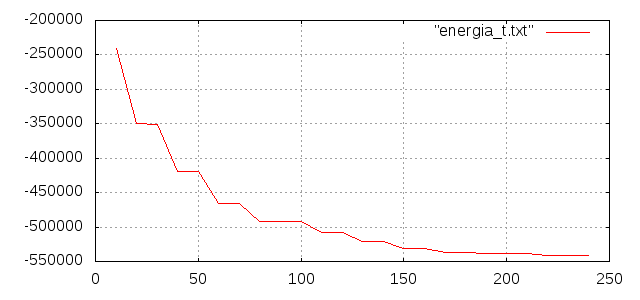
\includegraphics[scale=.4]{E-0-1-0-precavido.png}
\caption{E(t) con T nula}
\end{figure}
\begin{figure}
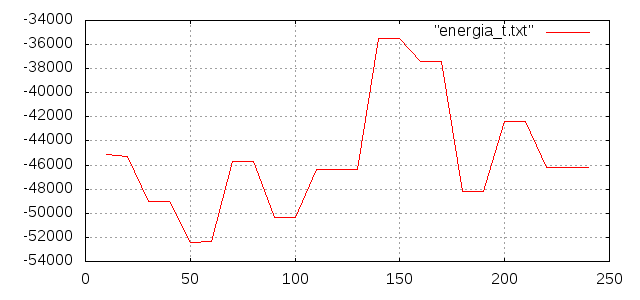
\includegraphics[scale=.4]{E-10000-1-0-precavido.png}
\caption{E(t) con T elevada}
\end{figure}

En la figura 3, el sistema se ordena f\'acilmente. En la 4, al sistema le cuesta m\'as ordenarse.

\begin{figure}
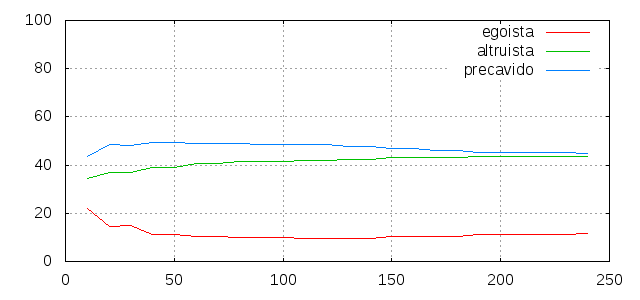
\includegraphics[scale=.4]{p-0-1-0-precavido.png}
\caption{Proporciones para T nula}
\end{figure}
\begin{figure}
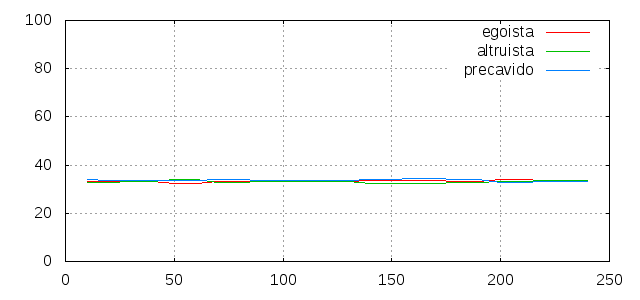
\includegraphics[scale=.4]{p-10000-1-0-precavido.png}
\caption{Proporciones para T alta}
\end{figure}

Puede verse que en la figura 3 el sistema evoluciona hacia cierta distribuci\'on de los estados, mientras que en la 4 el sistema tiende a la equiprobabilidad de los estados (33\%).

En estos casos hay que predecir c\'omo interacuaran los estados entre si. Para este caso he imaginado que un egoista junto a otro egoista no sera producente. Un egoista al lado de un altruista saldr\'a ganando, y el segundo perdiendo, l\'ogicamente. Altruista-altruista funcionar\'a bien, pues saldr\'an ganando los dos. Luego he introducido al precavido, que lo que hace es no fiarse y dar solo si recibe algo, por lo que siempre gana. Junto al altruista ganan los dos, mientras que junto al egoista no pierde ninguno. Ser\'ia como una copia del vecino. Se puede ver que es la estrategia m\'as estable. Su presencia impulsa a los altruistas. Sin ellos el comportamiento ser\'ia distinto, como se muestra en la otra figura. Se ve en la figura 5 que la proporci\'on se va a 50\%, m\'as o menos (ganando los egoistas). He mantenido el estado precavido porque era m\'as f\'acil que volver a cambiar el programa a 2 estados. He hecho que desaparezca r\'apidamente con los factores.

\begin{figure}
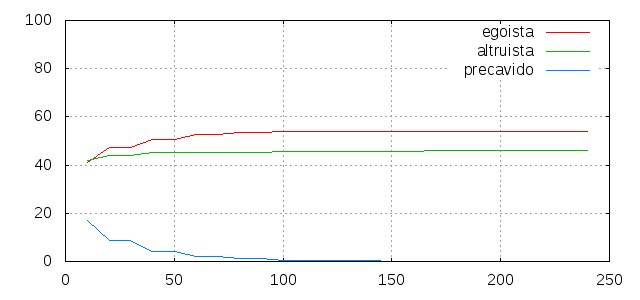
\includegraphics[scale=0.4]{p-0-1-0-2estados.png}
\caption{S\'olo egoista y altruista. Temperatura nula.}
\end{figure}


\subsection*{Sistema de cuatro niveles (egoista, altruista, copia, contrario)}

Ahora est\'an los comportamientos copia y contrario. Como par\'ametros he usado los mismos para egoista-copia que egoista-egoista, etc. copia-copia no gana ni pierde (al hacer el promedio) al igual que contrario-contrario. Se puede ver que la pareja egoista-copia son las m\'as estables en este caso, aunque la estrategia de copia es m\'as favorable. Observando las gr\'aficas 7,8, se puede ver que debe haber una transici\'on de fase entre esas temperaturas, pues en una hay tendencias y en la otra no. 

\begin{figure}
\includegraphics[scale=0.4]{proporciones-kbT0-A1-inf5-copia.png}
\caption{4 estados, T nula, tendencia hacia la copia}
\end{figure}

\begin{figure}
\includegraphics[scale=0.4]{proporciones-kbT10-A1-inf5-copia.png}
\caption{4 estados, T 10, tendencia hacia la copia}
\end{figure}

\begin{figure}
\includegraphics[scale=0.4]{proporciones-kbT100-A1-inf5-copia.png}
\caption{4 estados, T 100, tendencia hacia la copia}
\end{figure}

\section*{Conclusiones}

Podr\'ia seguir a\'nadiendo niveles, pero creo que ya se ha visto m\'as o menos la idea del programa (que no es m\'as que la del algoritmo de Metr\'opolis). He usado los ejemplos bas\'andome en el libro de Richard Dawkins, pero se puede usar cualquier otro ejemplo. En lo \'unico que hay que fijarse es en las interacciones entre estados. 


\section*{Posibles mejoras}

- Optimizando el programa se podr\'ian haber estudiado sistemas m\'as grandes y evoluciones durante m\'as pasos, por lo que ser\'a buena idea. 

- Se podr\'ian usar \textit{pipes} del sistema operativo para automatizar mejor el dibujado de los datos, pero no he tenido tiempo para estudiarme el tema.

- Para espines se pueden usar Booleans, lo que reduce la memoria usada (esto simplemente es cambiar la declaraci\'on en la plantilla).

- Tambi\'en se podr\'ia crear un diccionario, asociando a cada entero un estado, con lo que se cambiar\'ia el tipo base de string a int, reduciendo el uso de RAM.

- Como he explicado en la parte de simulaciones, se podr\'ia estudiar la temperatura cr\'itica haciendo una nueva rutina que cambie muchas veces los estados, mida la magnetizaci\'on y resetee el sistema para diferentes temperaturas.


\section*{Bibliograf\'ia}
- \textbf{''El gen egoista'' de Richard Dawkins}. Me he inspirado en \'el al realizar el ejemplo de egoistas, altruistas y precavidos. En su libro hay muchos m\'as ejemplos interesantes de c\'omo evolucionan los patrones de comportamiento en la naturaleza.

- \textbf{''Programaci\'on con C++''de  Al Stevens y Clayton Walnum, Ed Anaya}. Lo he usado como consulta para mirar las cosas que no recordaba de C++ y buscar informaci\'on sobre como hacer otras que no conoc\'ia.



\end{document}